\section{An initial overview of of the course}
\title[Initial overview]{Power Electronics Devices and Components}
 
\begin{frame}[plain]
    \titlepage
\end{frame}
%%%%%%%%%%%%%%%%%%%%%%%%%%%%%%%%%%%%%%%%%%%%%%%%%%%%%%%%%%%%%
%% Overview of the course %%
%%%%%%%%%%%%%%%%%%%%%%%%%%%%%%%%%%%%%%%%%%%%%%%%%%%%%%%%%%%%%
\begin{frame}
	\frametitle{Course Overview}
The course will be in 6 modules.
		\begin{itemize}
		  \item Module I: Introduction to Automation Technologies.
		  \item Module II: Sensor Technologies.
		  \item Module III: Signal Conditioning.
		  \item Module IV: Processors in Automation Systems.
		  \item Module V: Controllers and Communication.
%		  \item Module VI: Industrial communication systems.
		  \item Module VI: Actuators and Motion Systems.
		  \item Module VII: Testing and Validation.
		  \item Module VIII: Industrial Case Studies.
		\end{itemize}
\textbf{Pattern of class}: \\ Day: Tuesday, every week \\ 
Time: 8 am to 10 am (theory) and 10 am to 12 am (tutorial) (ideally but it can change) \\
Holidays: 23 Dec 2025, 30 Dec 2025, and 6 Jan 2026. %As required classes will be rescheduled. 
\end{frame}

%%%%%%%%%%%%%%%%%%%%%%%%%%%%%%%%%%%%%%%%%%%%%%%%%%%%%%%%%%%%%
%% Teaching Support Team %%
%%%%%%%%%%%%%%%%%%%%%%%%%%%%%%%%%%%%%%%%%%%%%%%%%%%%%%%%%%%%%
\begin{frame}
	\frametitle{The teaching team}
	\vspace{-0.5cm}
	\begin{columns}[t]
\centering
		\column[T]{0.33\textwidth}
		\begin{figure}
			\centering
				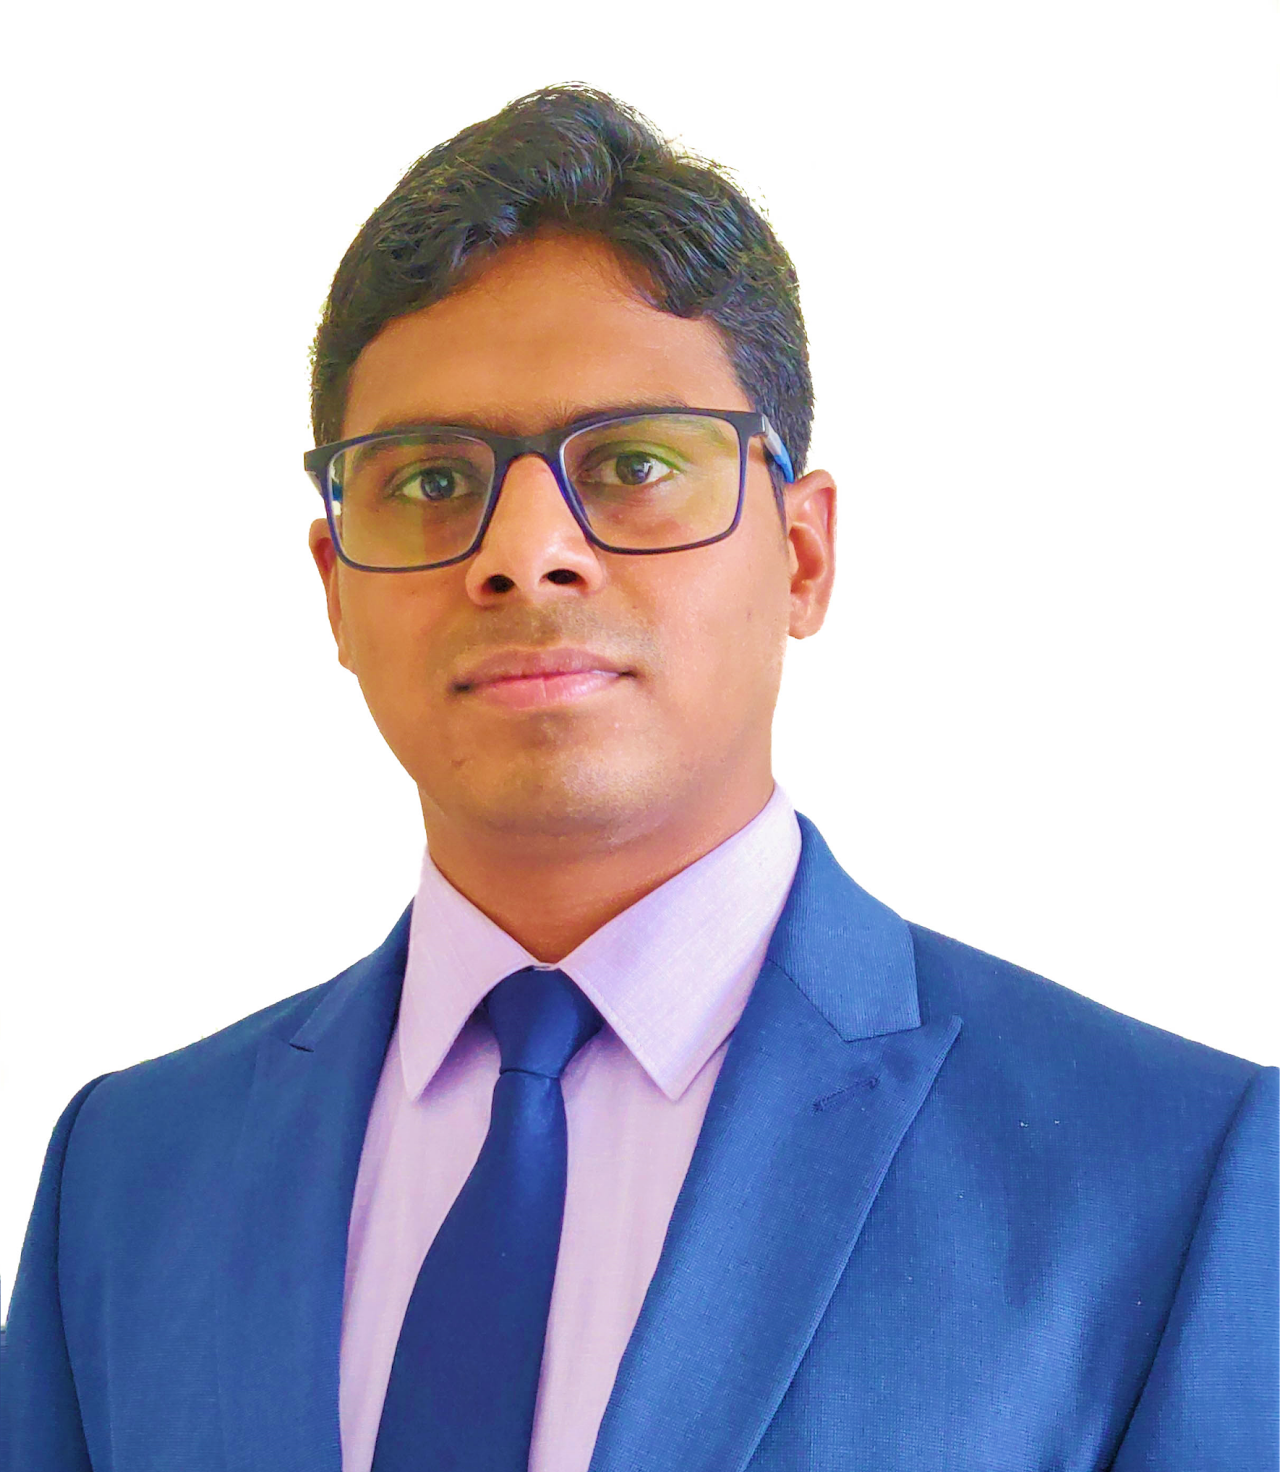
\includegraphics[height=2.5cm]{fig/lec01/Bikash.png}
				\caption*{Bikash Sah}
		\end{figure}
	
		\column[T]{0.33\textwidth}
		\begin{figure}
			\centering
				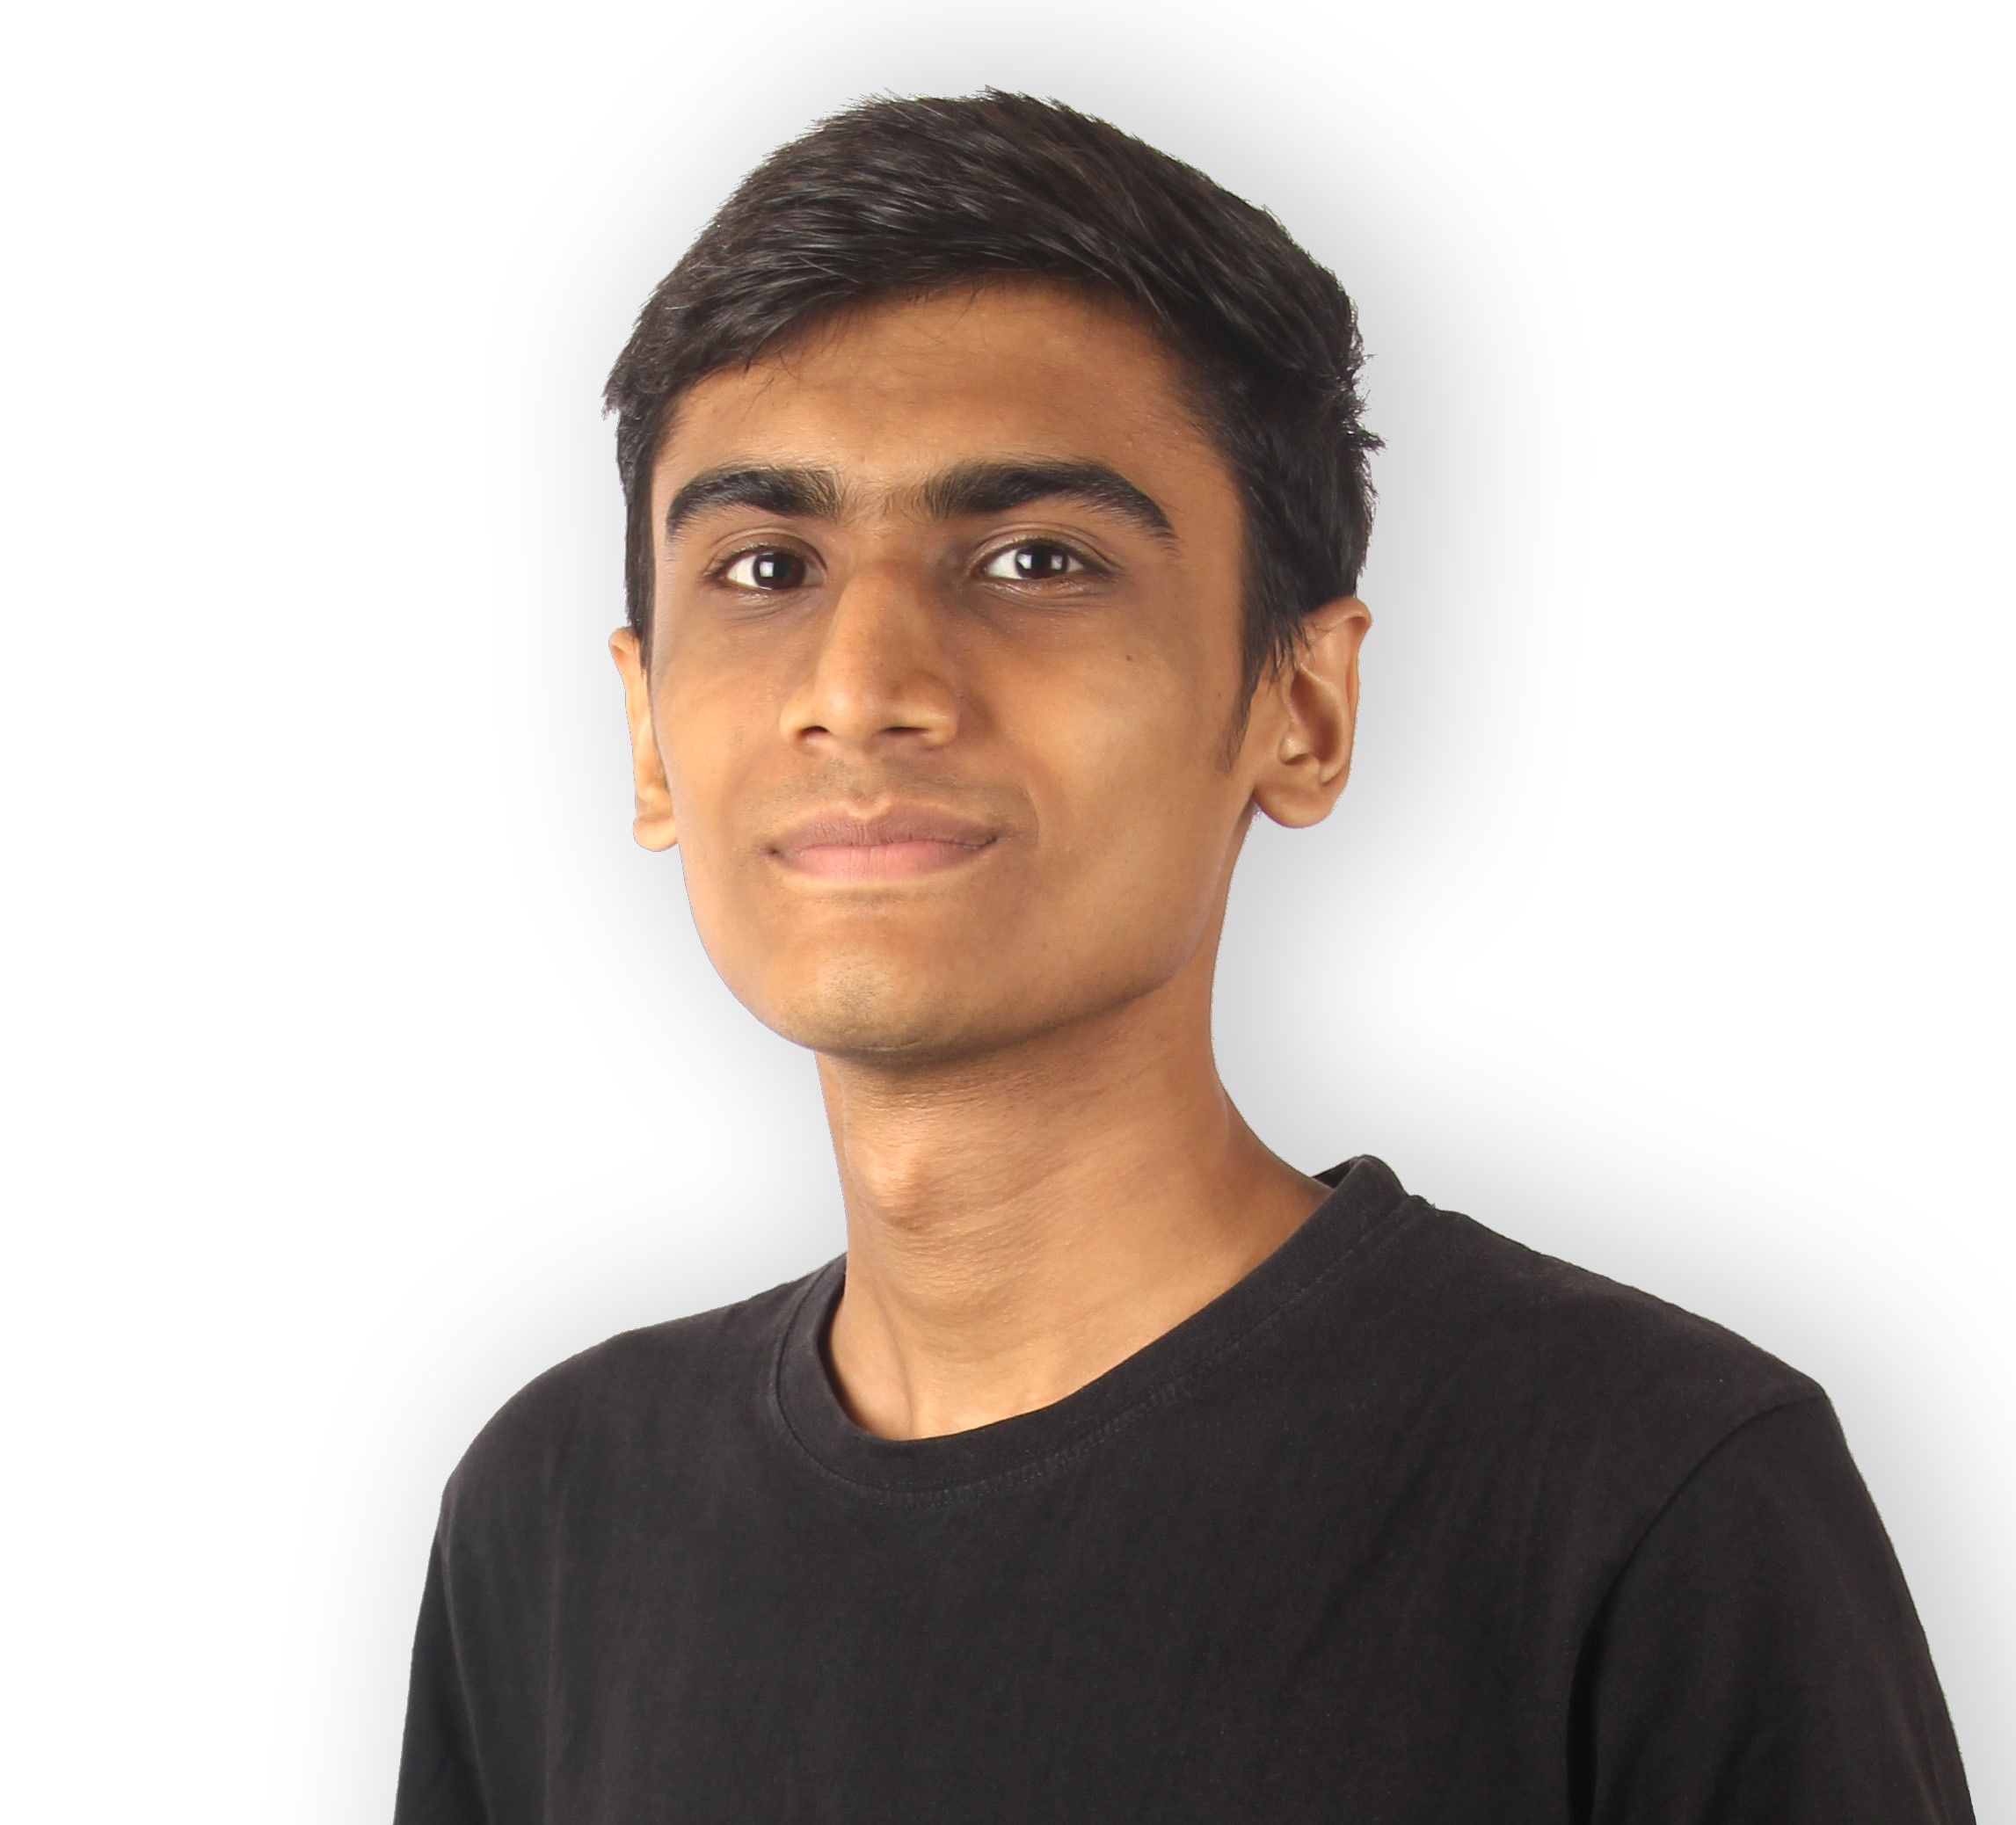
\includegraphics[height=2.5cm]{fig/lec01/Tatsat.jpg}
				\caption*{Tatsat Baldaniya}
		\end{figure}
		\column[T]{0.33\textwidth}
		\begin{figure}
			\centering
				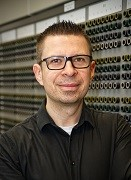
\includegraphics[height=2.5cm]{fig/lec01/pawel.jpg}
				\caption*{Pawel Malicki}
		\end{figure}		
	\end{columns}
	\vspace{-0.5cm}
	\begin{varblock}{Contact}
		\begin{itemize}
			\item Email: see \href{https://www.eti.uni-siegen.de/ias/}{chair's homepage}
			\item Offices: H-A building, 4th floor
			\item Individual appointments on request (remote or personally)
            \item Multiple relevant courses are offered by the Chair.  \href{https://www.eti.uni-siegen.de/ias/teaching/}{Check link!}
		\end{itemize}
	\end{varblock}
%** \small{Future follow-up courses are planned to be introduced in next semester- High Frequency Power Electronics, etc.}
	\end{frame}



%%%%%%%%%%%%%%%%%%%%%%%%%%%%%%%%%%%%%%%%%%%%%%%%%%%%%%%%%%%%%
%% Start %%
%%%%%%%%%%%%%%%%%%%%%%%%%%%%%%%%%%%%%%%%%%%%%%%%%%%%%%%%%%%%%
\begin{frame}
\center
\textbf{\huge{Module I: Introduction to Automation Technologies}}
\end{frame}

%%%%%%%%%%%%%%%%%%%%%%%%%%%%%%%%%%%%%%%%%%%%%%%%%%%%%%%%%%%%%
%% What is Electronics %%
%%%%%%%%%%%%%%%%%%%%%%%%%%%%%%%%%%%%%%%%%%%%%%%%%%%%%%%%%%%%%
\begin{frame}
	\frametitle{What are "Electronic Devices"?}
	\begin{columns}
		\begin{column}{0.5\textwidth}
			\begin{varblock}{Electronic Devices}
				Electronic devices are hardware components which leverage the property of materials to control the flow of electrons or charge.
			\end{varblock} \vspace{-0.5cm}		
			\begin{itemize}
				\item<2-> Have a long history of development- started with the invention of vaccum tube or Thermionic valve in 1904 by J.A. Fleming.
				\item<3-> The first transistor was invented in 1947 by J.Bardeen, W.H. Brattain and W.S. Shockley in Bell Labs.
				\item<4-> The first integrated circuit was invented in 1958 by J. Kilby and R. Noyce -- On and it goes
%				\item<5-> The first microprocessor was invented in 1971 by F. Faggin, T. Klein and H. Hoff in Intel.
%				\item<6-> The first microcontroller was invented in 1971 by F. Faggin, T. Klein and H. Hoff in Intel.
%				\item<7-> On and it goes- every day new devices are invented and developed.
			\end{itemize}
		\end{column}
		\begin{column}{0.5\textwidth}
			\begin{figure}
				\centering
				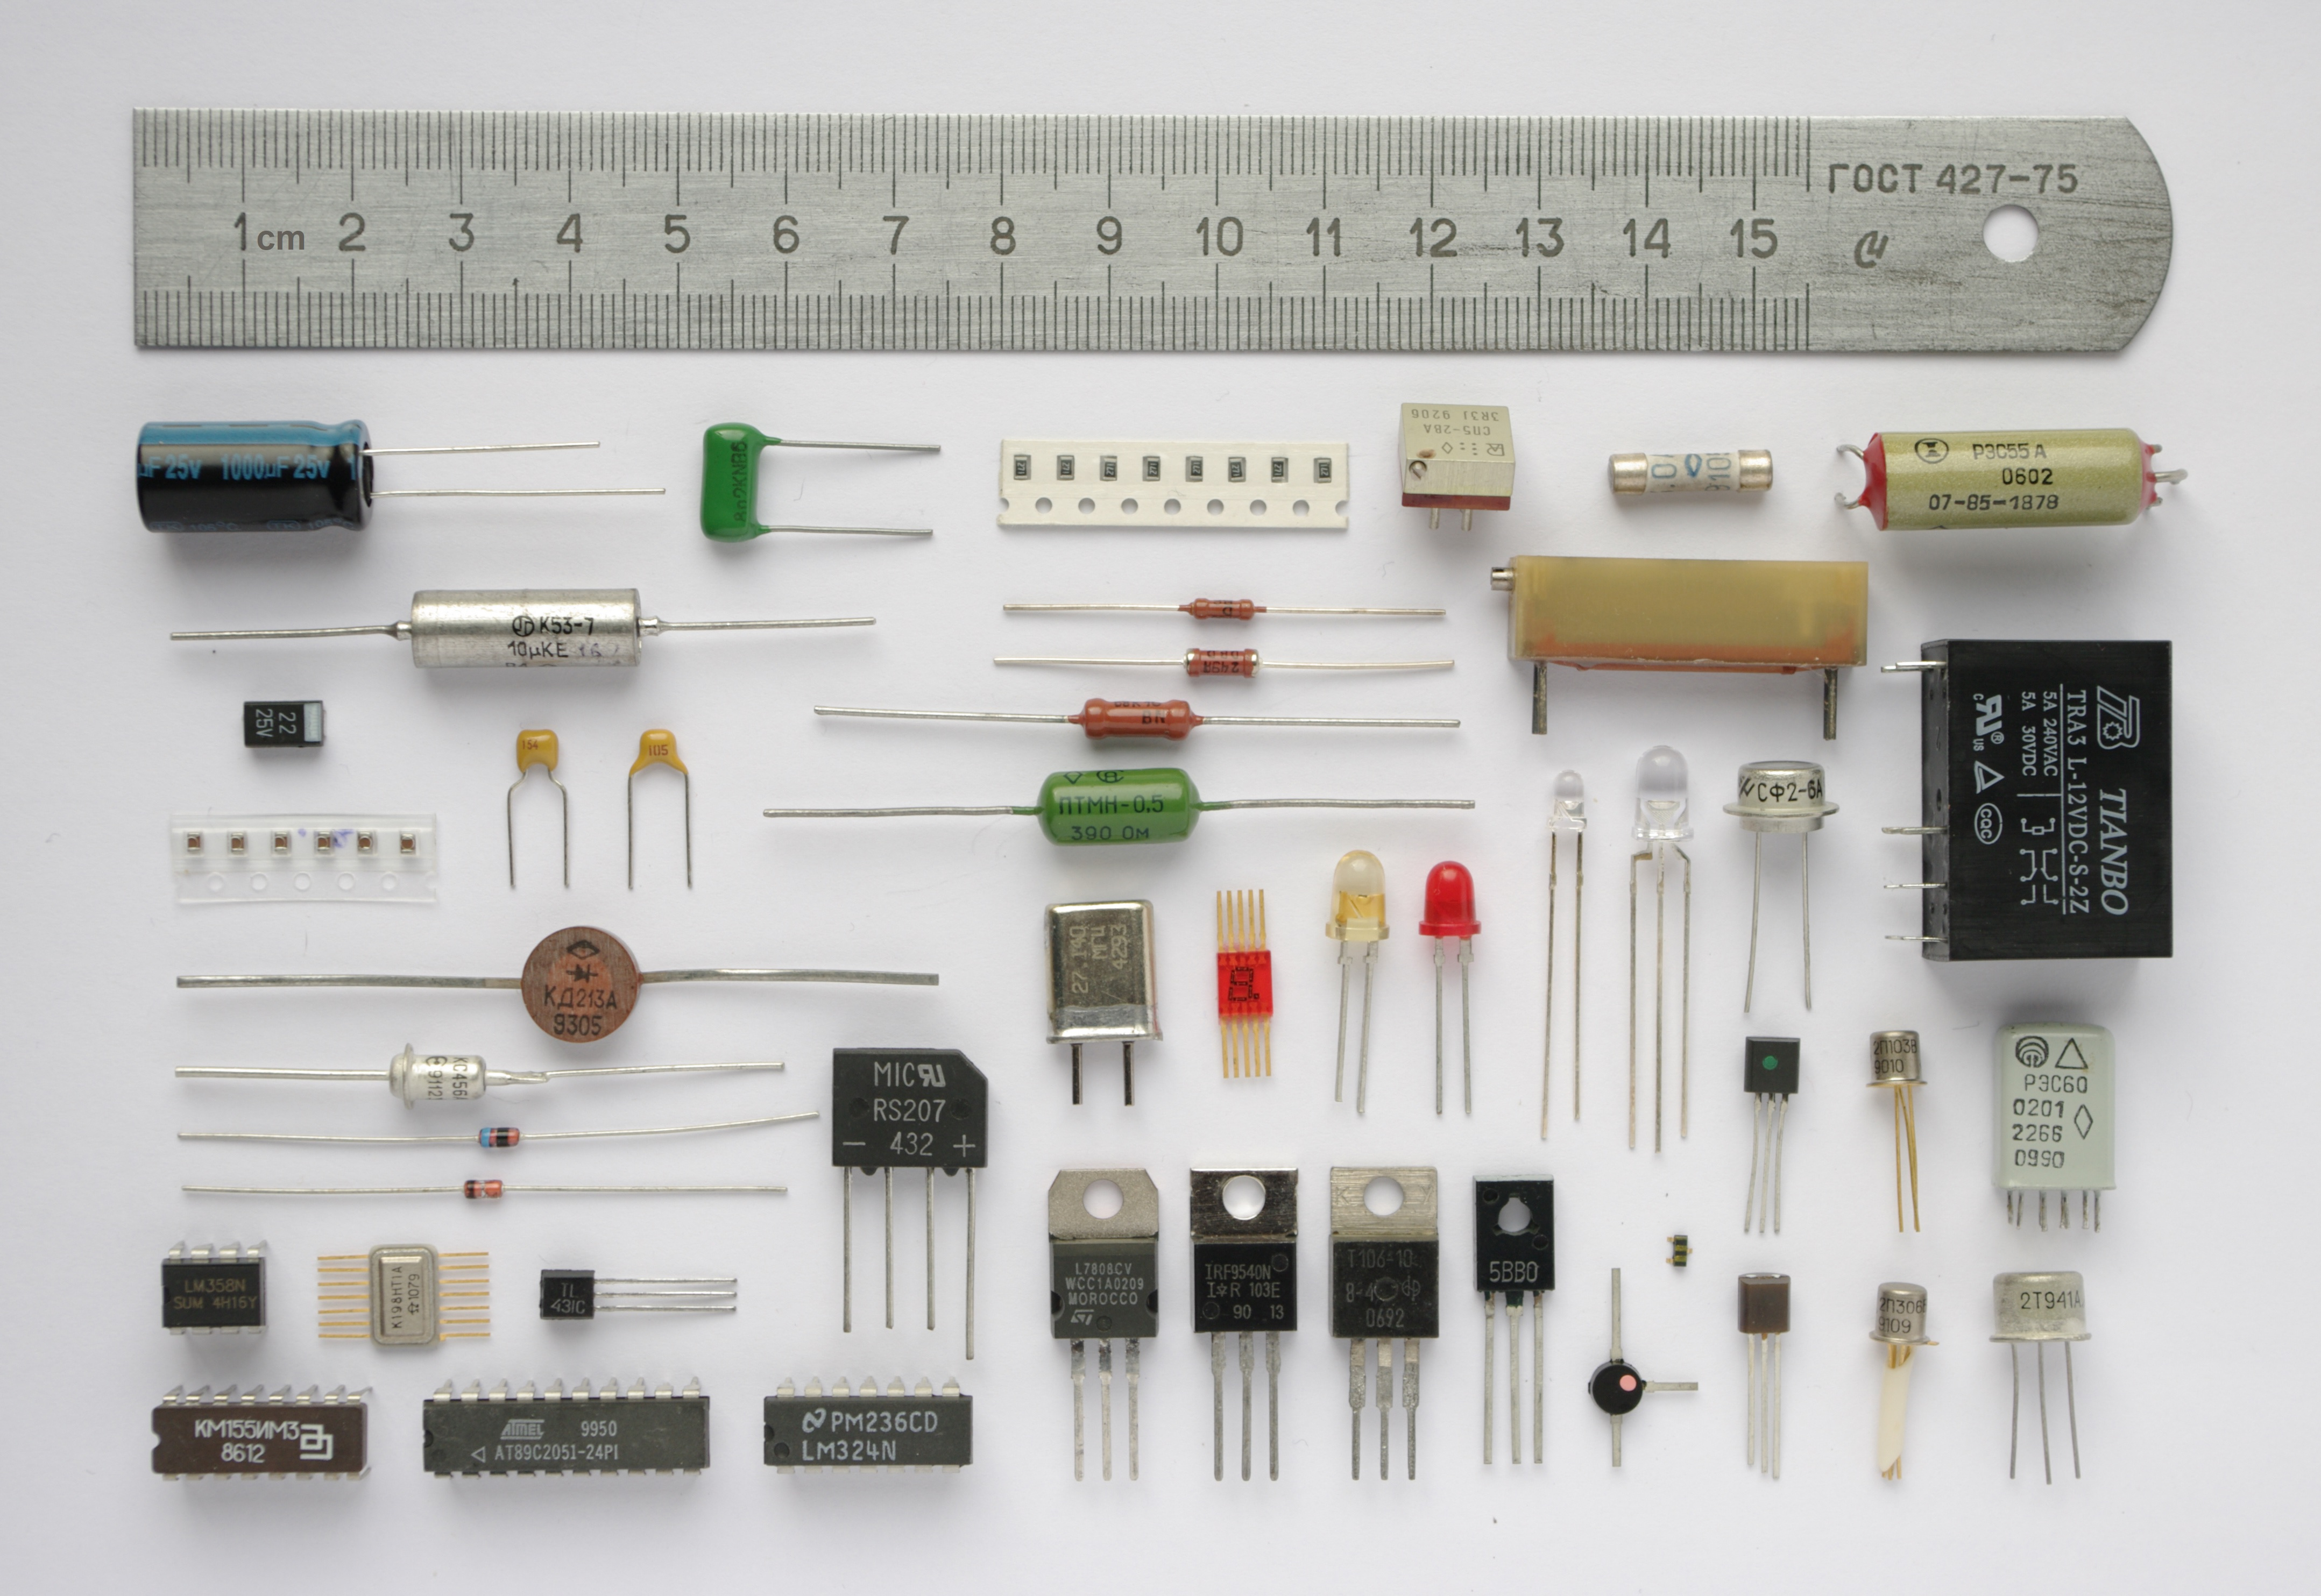
\includegraphics[scale= 0.05]{fig/lec01/Componentes.jpg}
				\caption{Example of electronic components (source: \href{https://commons.wikimedia.org/wiki/File:Componentes.JPG}{Wikimedia Commons}, Kae, public domain)}
			\end{figure}
		\end{column}
		\end{columns}
\end{frame}


%%%%%%%%%%%%%%%%%%%%%%%%%%%%%%%%%%%%%%%%%%%%%%%%%%%%%%%%%%%%%
%% Necessary prior knowledge %%
%%%%%%%%%%%%%%%%%%%%%%%%%%%%%%%%%%%%%%%%%%%%%%%%%%%%%%%%%%%%%
\begin{frame}
	\frametitle{Necessary prior knowledge for this course}
	You should have a basic understanding of the following topics:
	\begin{itemize}
		\item Basic electrical engineering knowledge (e.g., Ohm's law, Kirchhoff's laws, etc.)
		\item Basic understanding of physics in electronics
		\item Algebra and complex numbers
		\item Basic signal theory knowledge (e.g., Fourier series, Laplace transform)
		\item No advanced knowledge of semiconductors or programming is needed — this course builds those concepts from scratch and applies them to real systems.
	\end{itemize}
	\vspace{0.5cm}
	\onslide<2->What we will \underline{not} cover, but you do not need to know (covered in separate courses):
	\begin{itemize}
		\item Power converter circuits and topologies.
		\item Power electronics in depth involving analysis and controller design. 
	\end{itemize}
\end{frame}

%%%%%%%%%%%%%%%%%%%%%%%%%%%%%%%%%%%%%%%%%%%%%%%%%%%%%%%%%%%%%
%% Recommended reading %%
%%%%%%%%%%%%%%%%%%%%%%%%%%%%%%%%%%%%%%%%%%%%%%%%%%%%%%%%%%%%%
\begin{frame}
	\frametitle{Recommended reading}
	\begin{itemize}
		\item Baliga, B. Jayant. Fundamentals of power semiconductor devices. Springer Science \& Business Media, 2010.
		\item Lutz, Josef, Heinrich Schlangenotto, Uwe Scheuermann, and Rik De Doncker. "Semiconductor power devices." Physics, characteristics, reliability 2 (2011).
		\item Baliga, B. Jayant, ed. Wide Bandgap Semiconductor Power Devices: Materials, Physics, Design, and Applications. Woodhead Publishing, 2018.
		\item K. Niayesh, M. Runde, "Power Switching Components Theory, Applications and Future Trends", 1. Ed., Springer, 2018.
	\end{itemize}
\end{frame}